\section{ESTIMAÇÃO}
	\paragraph{}
    	Existem vários casos que podem ser estimados. Sabe-se o parâmetros dos itens, e não as habilidades dos respondentes, 
    	Sabe-se as habilidades dos estudantes mas não sabe-se os parâmetros dos itens,e o caso mais comum quando não sabemos nem os parâmetros dos itens nem as habilidades dos respondentes, neste caso faz-se a estimação conjunta de parâmetros e habilidades.
	\par
	    Assim estimar os parâmetros dos itens tem como significado encontrar os valores dos parâmetros da função características do item que se ajustem aos dados, ou seja, encontrar os valores dos parâmetros a,b e c e $\theta$.
	\begin{figure}[!h]
	    \centering
	    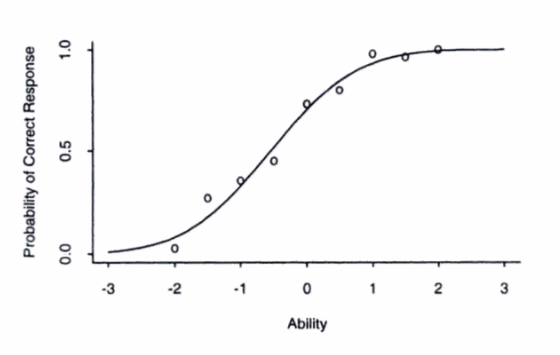
\includegraphics[width=0.6\linewidth]{img/proporcao}
	    \caption{Proporção de respostas corretas dada a um item}
	    \label{fig:proporcao}
	\end{figure}
	
	\subsection{Máxima-verossimilhança}
	\paragraph{}
	    O princípio de máxima verossimilhança(MVM) o procedimento usado para se obtenção de estimadores em estatística. Consideremos uma população e uma variável aleatória $X$, relacionada a essa população, com função de probabilidade (se é uma variável aleatória discreta) ou função densidade de probabilidade (se  é uma variável aleatória contínua) no nosso caso a função característica do item(CCI) , sendo  o parâmetro desconhecido. Retiremos uma amostra aleatória simples de , de tamanho $n$, e sejam  os valores efetivamente observados.\par
	    A função de verossimilhança  é definida por:
	\begin{equation}
	    L(\theta; x_1,x_2,...,x_n) = f(x_1;\theta) \times ... f(x_n;\theta) = \prod_{i = 1}^{n} f(x_i;\theta)
	    \label{fun:vero}
	\end{equation}
	    Onde $f(x_n;\theta)$ é a função de densidade de probabilidade, que deve ser interpretada como uma função de $ \theta $. O estimador de máxima verossimilhança de $ \theta $ é o valor que maximiza $ L(\theta;x_1,\ldots,x-n) $
	    Em muitos casos, o estimador de máxima verossimilhança pode ser encontrado seguindo os passos abaixo:\\
    \begin{enumerate}
        \item Encontrar a função de verossimilhança(\ref{fun:vero});
        \item Aplicar a função log;
        \item Derivar em relação ao parâmetro $ \theta , x_1,x_2...x_n$;
        \item Igualar o resultado a zero.
        \item Verificar que este estimador é ponto de máximo.
    \end{enumerate}
    \paragraph{}
	    Em outras palavras, tendo-se um conjunto de dados e um modelo estatístico, o método de máxima verossimilhança estima os valores dos diferentes parâmetros do modelo estatístico de maneira a maximizar a probabilidade dos dados observados (isto é, busca parâmetros que maximizem a função de verossimilhança). O método de máxima verossimilhança apresenta-se como um método geral para estimação de parâmetros, principalmente no caso de distribuições normais. Assim para encontrarmos o valor dos dados que maximizam a função de MV, precisamos derivar a função de MV e encontrar o valor que são raízes desta função derivada.
	\subsection{Estimação para uma única população}
	\cite{George} 
    	Considerando no caso de N indivíduos, $1 < j < N$, respondendo a I itens, $1 < i < I$, onde cada resposta é: $U_{ji} = 1$ como correta ou $U_{ji} = 0$ incorreta . Utilizando o MVM podemos estimar os parâmetros dos itens no modelo logístico de 3 parâmetros, temos as seguintes definições:
	\paragraph{}
	\begin{table}[!h]
	    \centering
    	\begin{tabular}{rl}
    	    $U_j = (U_{j1},U_{j2},...,U_{jI})$ & sendo o vetor de respostas do respondente j\\ 
        	$\zeta = (\zeta_1,\zeta_2,...,\zeta_I)$ & vetor de dos parâmetros dos itens\\
    	    $\theta = (\theta_1,\theta_2,...,\theta_N)$ & vetor de habilidades dos respondentes
    	\end{tabular}
	\end{table}
  
	$$
	U_{ij} = \left\{
	\begin{array}{ll}
    	1, resposta \quad correta,\\
    	0, resposta \quad incorreta.
    	
    	\end{array}\right.
	$$
	
	\subsubsection{Encontrando a função de verossimilhança}
	\paragraph{}
	    Para fazer a estimação dos parâmetros dos itens, temos que encontrar a função de máxima-verossimilhança, ver definição(\ref{fun:vero}), sendo o produto das probabilidades dos $N$ indivíduos responder corretamente o item $i$.
	\begin{eqnarray}
		L(\zeta) &=& \prod_{j = 1}^{n}P_i(U_{j.} = u_{j.}|\theta_j)\\
		L(\zeta) &=& \prod_{j=1}^{N}\prod_{i = i}^{I}P(U_{ij} = u_{ij}|\theta_j,\zeta_i)
	\end{eqnarray}
	
	\begin{eqnarray}
		P_{ji} &=& P(U_{ji} = 1|\theta_j,\zeta_i)\\
		Q_{ji} &=& 1 - P_{ji}
	\end{eqnarray}
	
	temos:
	
	\begin{eqnarray}
		P(U_{ji} = u_{ji}|\theta_j,\zeta_i) &=& P(U_{ji} = 1|\theta_j,\zeta_i)^{u_{ji}}P(U_{ji} = 0|\theta_j,\zeta_i)^{1 - u_{ji}}\\
		& = & P_{ji}^{u_{ji}}Q_{ji}^{1 - u_{ji}}
	\end{eqnarray}
	assim:
	
	$$
	L(\zeta) = \displaystyle\prod_{j = 1}^N\displaystyle\prod_{i = 1}^{I}P_{ji}^{u_{ji}}Q_{ji}^{1 - u_{ji}}
	$$
	
	\subsubsection{Aplicando a função log}
	\paragraph{}
	    Como devemos derivar a função de verossimilhança, derivar o produtorio de $N \times i$ termos é uma tarefa árdua, então podemos usar o artificio matemático de aplicar o logaritimo a $L(\zeta)$ visto que os mesmos parâmetros que maximizam a função $L(\zeta)$ são os mesmos para $\log(L(\zeta))$
	
	seguindo log-verossimilhança\\
	$$
	\log L(\zeta) = \displaystyle\sum_{j = 1}^{N}\displaystyle\sum_{i = 1}^{I}\{u_{ji}\log P_{ji} + (1 - u_{ji})\log Q_{ji}\}
	$$
	Os Estimadores de Máxima verossimilhança (EMV) de $\zeta_i$ , i = 1,..., I, são os valores que maximizam a verossimilhança, ou equivalente, são as soluções da equação:
	\subsubsection{Igualando a função igual a zero}
	$$
	\displaystyle\frac{\partial\log L(\zeta)}{\partial\zeta_i} = 0
	$$
	
	\begin{eqnarray}
		\displaystyle\frac{\partial\log L(\zeta)}{\partial\zeta_i} & = &\displaystyle\sum_{j = 1}^{N}\left\{u_{ji}\displaystyle\frac{\partial(\log P_{ji})}{\partial\zeta_i} + (1 - u_{ji})\displaystyle\frac{\partial(\log Q_{ji})}{\partial\zeta_i}\right\}\\
		& = & \displaystyle\sum_{j = 1}^{N}\left\{
		u_{ji}\displaystyle\frac{1}{P_{ji}}\left(\displaystyle\frac{\partial P_{ji}}{\partial \zeta_i}\right) - (1 - u_{ji})\displaystyle\frac{1}{Q_{ji}}\left(\displaystyle\frac{\partial P_{ji}}{\partial \zeta_i}\right)
		\right\}\\
		& = & \displaystyle\sum_{j = 1}^{N}\left\{u_{ji}\displaystyle\frac{1}{P_{ji}} - (1 - u_{ji})\displaystyle\frac{1}{Q_{ji}}\right\}\left(\displaystyle\frac{\partial P_{ji}}{\partial \zeta_i}\right)\\
		& = & \displaystyle\sum_{j = 1}^{N}
		\left\{
		\displaystyle\frac{u_{ji} - P_{ji}}{P_{ji}Q_{ji}}
		\right\}				
		\left(
		\displaystyle\frac{\partial P_{ji}}{\partial \zeta_i}
		\right)
	\end{eqnarray}
	
	por conveniência
	
	$$
	    W_{ji} = \displaystyle\frac{P_{ji}^{*}Q_{ji}^{*}}{P_{ji}Q_{ji}}
	$$
	
	onde,
	
	$$
	    P_{ji}^{*} = \{1 + e^{-Da_i(\theta_j - b_i)}\}^{-1} \quad  \mbox{e} \quad Q_{ji}^{*} = 1 - P_{ji}^{*}
	$$
	assim podemos escrever
	$$
	    \displaystyle\frac{\partial\log L(\zeta)}{\zeta_i} = \displaystyle\sum_{j = 1}^{N}
	    \left\{
	    (u_{ji} - P_{ji})\displaystyle\frac{W_{ji}}{P_{ji}^{*}Q_{ji}^{*}}			
	    \right\}
	    \left(
	    \displaystyle\frac{\partial P_{ji}}{\partial \zeta_i}
	    \right)
	$$
	para obter os parâmetros serão necessários:
	\begin{eqnarray}
		\displaystyle\frac{\partial P_{ji}}{\partial a_i} &=& D(1 - c_i)(\theta_j - b_i)P_{ji}^{*}Q_{ji}^{*}\\
		\displaystyle\frac{\partial P_{ji}}{\partial b_i} &=& -Da_i(1 -c_i)P_{ji}^{*}Q_{ji}^{*}\\
		\displaystyle\frac{\partial P_{ji}}{\partial c_i} &=& Q_{ji}^{*}
	\end{eqnarray}
	para o parâmetro de discriminação
	\begin{eqnarray}
		\displaystyle\frac{\partial \log(\zeta)}{\partial a_i} & = & \sum_{j = 1}^{N}\left\{
		(u_{ji} - P_{ji})\left(\displaystyle\frac{\partial P_{ji}}{\partial a_i}\right)\displaystyle\frac{W_{ji}}{P_{ji}^{*}Q_{ji}^{*}}
		\right\}\\
		&=& \sum_{j = 1}^{N}\left\{
		(u_{ji} - P_{ji})D(1 - c_i)(\theta_j - b_i)P_{ji}^{*}Q_{ji}^{*}\displaystyle\frac{W_{ji}}{P_{ji}^{*}Q_{ji}^{*}}
		\right\}\\
		& = & D(1 - c_i)\sum_{j = 1}^{N}(u_{ji} - P_{ji})(\theta_j - b_i)W_{ji}		
	\end{eqnarray}		
	
	parâmetro de dificuldade\\
	
	\begin{eqnarray}
		\displaystyle\frac{\partial \log(\zeta)}{\partial b_i} & = & \sum_{j = 1}^{N}\left\{
		(u_{ji} - P_{ji})\left(\displaystyle\frac{\partial P_{ji}}{\partial b_i}\right)\displaystyle\frac{W_{ji}}{P_{ji}^{*}Q_{ji}^{*}}
		\right\}\\
		&=& \sum_{j = 1}^{N}\left\{	
		(u_{ji} - P_{ji})(-1)Da_{i}(1 - c_i)P_{ji}^{*}Q_{ji}^{*}\displaystyle\frac{W_{ji}}{P_{ji}^{*}Q_{ji}^{*}}
		\right\}\\
		& = & -Da_{i}(1 - c_i)\sum_{j = 1}^{N}(u_{ji} - P_{ji})W_{ji}
	\end{eqnarray}		
	parâmetro acaso\\
	\begin{eqnarray}
		\displaystyle\frac{\partial \log(\zeta)}{\partial c_i} & = & \sum_{j = 1}^{N}\left\{
		(u_{ji} - P_{ji})\left(\displaystyle\frac{\partial P_{ji}}{\partial c_i}\right)\displaystyle\frac{W_{ji}}{P_{ji}^{*}Q_{ji}^{*}}
		\right\}\\
		&=& \sum_{j = 1}^{N}\left\{	
		(u_{ji} - P_{ji})Q_{ji}^{*}\displaystyle\frac{W_{ji}}{P_{ji}^{*}Q_{ji}^{*}}
		\right\}\\
		&=& \sum_{j = 1}^{N}\left\{	
		(u_{ji} - P_{ji})\displaystyle\frac{W_{ji}}{P_{ji}^{*}}
		\right\}\\
	\end{eqnarray}
	\subsubsection{Método de Newton-Raphson}
	\paragraph{}
        O Método de Newton-Rapshon na forma matricial verifica se o conjunto de parâmetros é ponto de máximo, Assim:\\
	    Seja $l(\zeta) = \log L(\zeta)$ a log-verossimilhança, onde $\zeta = (\zeta_1,\zeta_2,...,\zeta_I)$ com $\zeta_i = (a_i,b_i,c_i)$
	    os valores inicias são $\hat{\zeta}^{(0)} = (a_i^{(0)},b_i^{(0)},c_i^{(0)})$
	
    	a estimativa para $l(\zeta) = \log L(\zeta)$ será 
	    $\hat{\zeta}^{(1)} = \hat{\zeta}^{(0)} + \Delta\hat{\zeta}_i^{(0)}$
	    ou seja\\
	\begin{eqnarray}
		\hat{a}_i^{(1)} & = & \hat{a}_i^{(0)} + \Delta\hat{a}_i^{(0)}\\
		\hat{b}_i^{(1)} & = & \hat{b}_i^{(0)} + \Delta\hat{b}_i^{(0)}\\
		\hat{c}_i^{(1)} & = & \hat{c}_i^{(0)} + \Delta\hat{c}_i^{(0)}
	\end{eqnarray}
	Onde:\\
	
	$\Delta\hat{a}_i^{(0)}$,$\Delta\hat{b}_i^{(0)}$,$\Delta\hat{c}_i^{(0)}$ são os erros de aproximação.\\
	Usando a expansão de Taylor de $\displaystyle\frac{\partial l(\zeta)}{\partial \zeta_i}$\\
	\begin{eqnarray}
		\displaystyle\frac{\partial l(\zeta)}{\partial a_i} & = & \displaystyle\frac{\partial l(\hat{\zeta}_i^{(0)})}{\partial a_i} + \Delta\hat{a}_i^{(0)} \displaystyle\frac{\partial^2 l(\hat{\zeta}_i^{(0)})}{\partial a_i^2} + \Delta\hat{b}_i^{(0)} \displaystyle\frac{\partial^2 l(\hat{\zeta}_i^{(0)})}{\partial a_i \partial b_i} + 
		\Delta\hat{c}_i^{(0)} \displaystyle\frac{\partial^2 l(\hat{\zeta}_i^{(0)})}{\partial a_i \partial c_i} + R_{a_i}(\hat{\zeta}_i^{(0)}) \nonumber\\
		\displaystyle\frac{\partial l(\zeta)}{\partial b_i} & = & \displaystyle\frac{\partial l(\hat{\zeta}_i^{(0)})}{\partial b_i} + \Delta\hat{b}_i^{(0)} \displaystyle\frac{\partial^2 l(\hat{\zeta}_i^{(0)})}{\partial b_i^2} + \Delta\hat{b}_i^{(0)} \displaystyle\frac{\partial^2 l(\hat{\zeta}_i^{(0)})}{\partial b_i \partial a_i} + \Delta\hat{c}_i^{(0)} \displaystyle\frac{\partial^2 l(\hat{\zeta}_i^{(0)})}{\partial b_i \partial c_i} + R_{b_i}(\hat{\zeta}_i^{(0)}) \nonumber\\
		\displaystyle\frac{\partial l(\zeta)}{\partial c_i} & = & \displaystyle\frac{\partial l(\hat{\zeta}_i^{(0)})}{\partial c_i} + \Delta\hat{a}_i^{(0)} \displaystyle\frac{\partial^2 l(\hat{\zeta}_i^{(0)})}{\partial c_i^2} + \Delta\hat{b}_i^{(0)} \displaystyle\frac{\partial^2 l(\hat{\zeta}_i^{(0)})}{\partial c_i \partial a_i } + \Delta\hat{c}_i^{(0)} \displaystyle\frac{\partial^2 l(\hat{\zeta}_i^{(0)})}{\partial c_i \partial b_i}+ R_{c_i}(\hat{\zeta}_i^{(0)}) \nonumber
	\end{eqnarray}
	
	$$
	\displaystyle\frac{\partial l(\zeta_i)}{\partial a_i} = \displaystyle\frac{\partial l(\zeta_i)}{\partial b_i} = \displaystyle\frac{\partial l(\zeta_i)}{\partial c_i} = 0
	$$
	
	usando a notação \\
	
	\begin{eqnarray}
		L_1 = \displaystyle\frac{\partial l(\hat{\zeta}_i^{(0)})}{\partial a_i} \quad L_{11} =  \displaystyle\frac{\partial^2 l(\hat{\zeta}_i^{(0)})}{\partial a_i^2} \quad L_{12}  = \displaystyle\frac{\partial^2 l(\hat{\zeta}_i^{(0)})}{\partial a_i \partial b_i} \quad L_{13} = \displaystyle\frac{\partial^2 l(\hat{\zeta}_i^{(0)})}{\partial a_i \partial c_i} \nonumber\\
		L_2 = \displaystyle\frac{\partial l(\hat{\zeta}_i^{(0)})}{\partial b_i} \quad L_{21} = \displaystyle\frac{\partial^2 l(\hat{\zeta}_i^{(0)})}{\partial b_i^2} \quad L_{22} = \displaystyle\frac{\partial^2 l(\hat{\zeta}_i^{(0)})}{\partial b_i \partial a_i} \quad L_{23} =  \displaystyle\frac{\partial^2 l(\hat{\zeta}_i^{(0)})}{\partial b_i \partial c_i}\nonumber\\
		L_3 = \displaystyle\frac{\partial l(\hat{\zeta}_i^{(0)})}{\partial c_i} \quad L_{31} = \displaystyle\frac{\partial^2 l(\hat{\zeta}_i^{(0)})}{\partial c_i^2} \quad L_{32} = \displaystyle\frac{\partial^2 l(\hat{\zeta}_i^{(0)})}{\partial c_i \partial a_i } \quad L_{33} = \displaystyle\frac{\partial^2 l(\hat{\zeta}_i^{(0)})}{\partial c_i \partial b_i} \nonumber
	\end{eqnarray}
	Dezprezando os restos
	
	\begin{eqnarray}
		0 &=& L_1 + L_{11}\Delta\hat{a}_i^{(0)} + L_{12}\Delta\hat{b}_i^{(0)} + L_{13}\Delta\hat{c}_i^{(0)}\\
		0 &=& L_2 + L_{21}\Delta\hat{a}_i^{(0)} + L_{22}\Delta\hat{b}_i^{(0)} + L_{23}\Delta\hat{c}_i^{(0)}\\
		0 &=& L_3 + L_{31}\Delta\hat{a}_i^{(0)} + L_{32}\Delta\hat{b}_i^{(0)} + L_{33}\Delta\hat{c}_i^{(0)}
	\end{eqnarray}
	
	forma matricial
	
	$$
	-\left(\begin{array}{c}
	L_1\\
	L_2\\
	L_3\\
	\end{array}\right) =  
	\left(\begin{array}{ccc}
	L_{11} & L_{12} & L_{13}\\
	L_{21} & L_{22} & L{23}\\
	L_{31} & L_{32} & L_{33}\\
	\end{array}\right)
	\left(\begin{array}{c}
	\Delta\hat{a}_i^{(0)}\\
	\Delta\hat{b}_i^{(0)}\\
	\Delta\hat{c}_i^{(0)}\\
	\end{array}\right)
	$$
	
	Resolvendo o sistema para $\Delta\hat{\zeta}_i^{(0)}$, teremos
	
	$$		
	\left(\begin{array}{c}
	\Delta\hat{a}_i^{(0)}\\
	\Delta\hat{b}_i^{(0)}\\
	\Delta\hat{c}_i^{(0)}\\
	\end{array}\right) =  
	-\left(\begin{array}{ccc}
	L_{11} & L_{12} & L_{13}\\
	L_{21} & L_{22} & L{23}\\
	L_{31} & L_{32} & L_{33}\\
	\end{array}\right)^{-1}
	\left(\begin{array}{c}
	L_1\\
	L_2\\
	L_3\\
	\end{array}\right)
	$$
	
	assim\\
	$$		
	\left(\begin{array}{c}
	\hat{a}_i^{(1)}\\
	\hat{b}_i^{(1)}\\
	\hat{c}_i^{(1)}\\
	\end{array}\right) = 	
	\left(\begin{array}{c}
	\hat{a}_i^{(0)}\\
	\hat{b}_i^{(0)}\\
	\hat{c}_i^{(0)}\\
	\end{array}\right) 
	-\left(\begin{array}{ccc}
	L_{11} & L_{12} & L_{13}\\
	L_{21} & L_{22} & L{23}\\
	L_{31} & L_{32} & L_{33}\\
	\end{array}\right)^{-1}
	\left(\begin{array}{c}
	L_1\\
	L_2\\
	L_3\\
	\end{array}\right)
	$$
	
	Este processo é repetido até que algum critério de parada seja alcançado. Por exemplo, até que
	$\Delta\hat{\zeta}_i^{(t)} = \hat{\zeta}_i^{(t)} - \hat{\zeta}_i^{(t - 1)}$
	
	para um número t de iterações
	ou que 	$\Delta\hat{\zeta}_i^{(t)}$ seja suficientemente pequeno.
	
	
	\subsection{Estimar habilidades}
	
	\begin{equation}
	\log L(\theta) = \displaystyle\sum\limits_{j = 1}^{n}\displaystyle\sum\limits_{i = 1}^{I}\{u_{ji}\log P_{ji} + (1 - u_{ji}) \log Q_{ji}\}
    \end{equation}
	\newpage
	\subsection{Outras metodologias de estimação}
	\paragraph{}
	    Pode-se ainda escolher outros metodos para obenção dos parametro dos itens.Tavares, mostra alguns ressaltando suas pontos positivos e negativos:\\
    	\textbf{Máxima Verossimilhança - MV :}\\
    	\textbf{negativo} - Para testes “longos” produz estimadores não viciados;\\
    	\textbf{positivo} - Não está definido para alguns padrões de resposta.\\
	    \textbf{Máxima Verossimilhança Marginal - MVM :}\\
	    \textbf{Bayesiano :}\\
	\par
	    Também existem os métodos para obtenção das habilidades dos indivíduos quando é sabido os parâmetros dos itens.\\
	    \textbf{Máxima Verossimilhança - MV}\\
	    \textbf{Bayesiano - EAP :}\\
	    \textbf{Bayesiano - MAP :}\\
	\par
	    Também podemos fazer estimação conjunta, quando  não sabemos nem os parâmetros dos itens e nem as habilidades dos indivíduos.\\
	    \textbf{Máxima Verossimilhança Conjunta - MVC :}\\
	
	Estimação conjunta: parâmetros dos itens e habilidades
	
	Uma vez terminada a calibração dos parâmetros, será feita a estimação
	das habilidades dos respondentes. O BILOG e o BILOG-MG têm implementados
	os métodos de estimação por máxima verossimilhança, por esperança a
	posteriori (EAP) e por máximo a posteriori (MAP). No método da máxima
	verossimilhança, as estimativas das habilidades dos respondentes são calculadas
	pelo método de Newton-Raphson, utilizando-se uma transformação linear
	do logito do percentual de acertos dos indivíduos como valores iniciais.
	
	\subsection{Escala de habilidade}
	\paragraph{}
	    Diferentemente da medida escore em um teste com I questões do tipo
	    certo/errado, que assume valores inteiros entre 0 e I, na TRI a habilidade pode
	    teoricamente assumir qualquer valor real entre $+\displaystyle\infty$ e $-\displaystyle\infty$. Assim, precisa-se estabelecer uma origem e uma unidade de medida para a definição da escala. Esses valores são escolhidos de modo a representar, respectivamente, o valor médio($\mu$) e o desvio-padrão($\sigma$) das habilidades dos indivíduos da população em estudo. Para os gráficos mostrados anteriormente, utilizou-se a escala com média igual a 0 e desvio-padrão igual a 1 que é utilizado para distribuições normais, que será representada por escala (0,1). Essa escala é bastante utilizada pela TRI, e nesse caso, os valores do parâmetro b variam (tipicamente) entre $-2$ e $+2$. Com relação ao parâmetro $a$, espera-se valores entre $0$ e $+2$, sendo que os valores mais apropriados de $a$ seriam aqueles maiores do que 1. Apesar da frequente utilização da escala (0,1), em termos práticos, não faz a menor diferença estabelecer-se estes valores ou outros quaisquer. O importante são as relações de ordem existentes entre seus pontos. Por exemplo, na escala (0,1) um indivíduo com habilidade 1,20 está 1,20 desvios-padrão acima da habilidade média. Este mesmo indivíduo teria a habilidade 248, e consequentemente estaria também 1,20 desvios-padrão acima da habilidade média, se a escala utilizada para esta população fosse a escala(200;40). Isto pode ser visto a partir da transformação de escala:
	\begin{eqnarray}
		1.\theta^* & = & \sigma \times \theta + u\\
		2 .b^* & = & \sigma \times b + u\\
		3. a^* & = & a/\sigma\\
		4. c^* & = & c\\
		5. P(U_i = 1|\theta) & = & P(U_i = 1|\theta*)\\
	\end{eqnarray}
	
	Na escala (0,1) um individuo com habilidade 1.20
	
	terá na escala (200;40)
	\begin{eqnarray}
    	 \theta^* & = & \sigma \times \theta + \mu \nonumber\\
    	 \theta^* & = & 40 \times 1,20 + 200 \nonumber\\
    	 \theta^* & = & 248 \nonumber\\
	 \end{eqnarray}
	\paragraph{}
	    De forma geral podemos expressar essa relação da seguinte maneira:\\
	\begin{eqnarray}
		P(U_{i} = 1,\theta) & = & c + (1-c)\displaystyle\frac{1}{1 + e^{-Da(\theta - b)}} | \theta = \theta^*, a = a^*, b = b*, c = c* \nonumber\\ 
		P(U_{i} = 1,\theta^*) & = & c^* + (1-c^*)\displaystyle\frac{1}{1 + e^{-Da^*(\theta^* - b^*)}} \nonumber\\
		P(U_{i} = 1,\theta^*) & = & c + (1-c)\displaystyle\frac{1}{1 + e^{-D(\frac{a}{\sigma})((\sigma \times \theta + u) - \sigma \times b + u)}}\nonumber\\
		P(U_{i} = 1,\theta^*) & = & c + (1-c)\displaystyle\frac{1}{1 + e^{-D(\frac{a}{\sigma})(\sigma(\theta - b)}} \nonumber\\
		P(U_{i} = 1,\theta^*) & = & c + (1-c)\displaystyle\frac{1}{1 + e^{-Da(\theta - b)}} \nonumber\\
		P(U_i = 1|\theta*) & = & P(U_i = 1|\theta) \nonumber
	\end{eqnarray}
	\subsection{Interpretação escala de habilidade}
	\paragraph{}
	    Uma vez que todos os parâmetros dos itens e que todas as habilidades dos respondentes — tanto individuais como populacionais — de todos os grupos avaliados estão numa mesma métrica, ou seja, quando todos os parâmetros envolvidos são comparáveis, pode-se então construir escalas de conhecimento interpretáveis.
	\paragraph{}
	    Definição de item âncora: Considere dois níveis âncora consecutivos Y e Z com Y $<$ Z. Dizemos que um determinado item é ancora para o nível Z se e somente se 3 condições abaixo forem satisfeitas simultaneamente: 
	
	\begin{eqnarray}
		P(U = 1 | \theta = Z) & \geq & 0,65 \\
		P(U = 1 | \theta = Y) & < & 0,50  \\
		P(U = 1 | \theta = Z) - P(U = 1 | \theta = Y) & < & 0,30
	\end{eqnarray}
	\paragraph{}
	    Em outras palavras, para um item ser âncora em um determinado nível âncora da escala, ele precisa ser respondido corretamente por uma grande 	proporção de indivíduos (pelo menos $65\%$) com este nível de habilidade e por uma proporção menor de indivíduos (no máximo $50\%$) com o nível de habilidade imediatamente anterior. Além disso, a diferença entre a proporção de indivíduos com esses níveis de habilidade que acertam a esse item deve ser de pelo menos $30\%$.
	
	avaliação\cite{Francisco}
	%https://ppgmat.ufersa.edu.br/wp-content/uploads/sites/58/2016/02/Disserta%C3%A7%C3%A3o-Francisco-Edmilson.pdf
	\newpage